\documentclass{article}
\usepackage{microtype}
\usepackage{graphicx}
\usepackage{booktabs}
\usepackage{hyperref}
\usepackage{icml2026}
\usepackage{amsmath,amssymb,mathtools,amsthm}
\usepackage[T1]{fontenc}
\newtheorem{theorem}{Theorem}
\newtheorem{proposition}[theorem]{Proposition}
\newtheorem{lemma}[theorem]{Lemma}
\newcommand{\ind}{\mathbf{1}}
\newcommand{\R}{\mathbb{R}}
\newcommand{\supp}{\operatorname{supp}}
\icmltitlerunning{Targeted Score Investment in Multi-Task Leaderboards}
\begin{document}
\twocolumn[
\icmltitle{Targeted Score Investment in Multi-Task Leaderboards:\\Feasibility, Aggregation, and Metric Dependence}
\begin{icmlauthorlist}
\icmlauthor{Anonymous Authors}{anon}
\end{icmlauthorlist}
\icmlaffiliation{anon}{Anonymous Institution}
\icmlcorrespondingauthor{Anonymous Authors}{anonymous@example.invalid}
\icmlkeywords{benchmark evaluation, leaderboard robustness, rank aggregation, counterfactual optimization}
\vskip 0.3in
]
\printAffiliationsAndNotice{}
\begin{abstract}
How many task scores must a developer improve to make a particular model first on a multi-task leaderboard? We study bounded, upward-only score interventions, explicitly not a model of training cost, under mean, median, and Borda aggregation. Monotonicity reduces minimum edited-task count to endpoint subset selection; threshold crossings characterize odd medians, while integer margin constraints account for both target gains and displaced Borda rivals. Experiments on fixed public matrices from HELM MMLU (79 models, 57 subjects) and Open LLM (4,576 configurations, six tasks) show that attainability and conditional edit count must be reported separately. For shared first, median needs fewer edits than mean on average at half-headroom ceilings but more on average at full-headroom ceilings on fixed jointly feasible nonwinner cohorts; for 64 of 77 HELM nonwinners, median nevertheless requires less total score gain despite editing more tasks. These results establish conditional rather than universal aggregation comparisons, with reproducible witnesses, numerical audits, and sensitivity analyses for ties, scaling, and competitor composition.
\end{abstract}

\section{Introduction}
Multi-task leaderboards compress a vector of measured behaviors into one ordering. When that ordering influences adoption and research attention, task-specific investment can have disproportionate value. A developer could prioritize data related to selected evaluations, improving some coordinates much more than others. Yet the resulting ranking change depends on how coordinates are aggregated, how much each can improve, and what is counted as investment.

A simple intuition says that medians should resist concentrated improvement because a large gain on one task cannot dominate the summary. That intuition is incomplete: resistance to one exceptionally large coordinate is not the same as the minimum number of coordinates needed to reach a particular rival. A median only needs enough threshold crossings; a mean needs a sufficient sum. If allowable gains are small, crossing several nearby thresholds may be cheaper in task count than closing a mean deficit. When gains are large, a mean deficit may be closed by fewer tasks. The distinction is also metric-dependent: editing more tasks can require less total score increase.

This paper gives an operational answer using only public scores. We hold the task panel and competitors' raw scores fixed, select a target, and find its smallest upward score intervention attaining first place. Equal-cost task edits define our primary investment metric. A ceiling parameter controls the allowed fraction of remaining score headroom. Mean and median aggregate scores directly; Borda aggregates within-task relative performance. Because editing one target also changes rival Borda totals, the latter comparison cannot use a fixed rival aggregate threshold.

\textbf{Scope boundary.} Our conclusions concern the geometry of published score tables, not the effectiveness or resource cost of training on benchmark-related data. There is no evidence here that any computed edit is attainable by training, that scores remain independent under real updates, or that any submitted model is contaminated. This limitation is fundamental, not repaired by optimizing the intervention more precisely.

The contributions are: (i) a precise bounded score-investment estimand separating attainability, minimum task count, and minimum magnitude; (ii) exact support characterizations and a finite Borda covering formulation, with a ceiling-independent plateau for feasible odd medians; and (iii) a two-snapshot empirical analysis showing ceiling-dependent comparisons on fixed target cohorts and strong count--magnitude disagreement. Small exact constructions rule out universal pairwise support dominance for shared first. We do not assert priority over all previous literature: the independent-reading constraint described in Appendix~\ref{app:restriction} deliberately limits our related-work coverage.

\section{Related Work}
\textbf{Benchmarks and aggregation.} MMLU supplies a broad collection of subject-level multiple-choice evaluations \citep{hendrycks2021mmlu}. HELM emphasizes standardized adaptation and multiple evaluation dimensions \citep{liang2023helm}. We use the public HELM MMLU export rather than conflating the original HELM suite with the MMLU subject matrix. The Benchmark Lottery demonstrates task-subset sensitivity and discusses cases in which mean and median rankings disagree \citep{dehghani2021benchmarklottery}. Our intervention instead keeps the task panel fixed and changes one target row. The task-as-voter perspective of \citet{lanctot2023evaluating} motivates an ordinal comparator, Borda, alongside cardinal rules. Their axiomatic discussion does not imply a universal ordering of score-edit costs.

\textbf{Incentives and leakage.} \citet{zhou2023benchmarkcheater} distinguish benchmark-related training from extreme test-set leakage and experimentally show that evaluation scores can change under these interventions. We do not reproduce such training or infer a score-to-resource response curve. The abstract of \citet{chen2026leaderboard} frames benchmark design and developer allocation as a strategic post-training game. Our optimization is a single-target, fixed-opponent structural diagnostic, not an equilibrium model. We rely only on that paper's abstract-level framing, not unverified assumptions or theorem statements. All citations were checked against permitted originals; no citation-graph expansion or thematic discovery search was used.

\section{Model and Investment Metrics}
Let $S\in[0,1]^{m\times n}$ contain higher-is-better scores for $m\ge2$ configurations on $n$ tasks. For target $i$, let $x_j=S_{ij}$ and permit
\begin{equation}
 x_j\le y_j\le c_j(\rho)=x_j+\rho(1-x_j),\quad 0<\rho\le1.
 \label{eq:ceiling}
\end{equation}
Only the target's raw scores change. The score ceiling $1$ is the natural perfect-score endpoint for the selected bounded metrics; $\rho$ is a hypothetical intervention constraint, not a fitted training efficiency. This box permits independent, arbitrary partial improvements and no regressions or spillovers. It is deliberately optimistic as a model of feasible intervention directions, but cannot be called a lower bound on real resources without further assumptions.

\subsection{Aggregation and Winning}
Mean is $A_\mu(s)=n^{-1}\sum_j s_j$. Median $A_{\rm med}$ is the middle order statistic for odd $n$, and the arithmetic average of the two middle statistics for even $n$. Each task receives equal weight. This is not sample-weighted MMLU accuracy and is not asserted to reproduce HELM's published headline aggregate.

For Borda, define doubled pair points
\begin{equation}
 q_{ij}=\sum_{r\ne i}\big(2\ind\{S_{ij}>S_{rj}\}+\ind\{S_{ij}=S_{rj}\}\big),
 \label{eq:borda}
\end{equation}
and total $B_i=\sum_jq_{ij}$. Dividing by $2n(m-1)$ would normalize to $[0,1]$ without changing the winner. Task ties receive half credit. After editing the target, all affected pair contributions are recomputed, including rivals' totals.

\emph{Shared first} means the target's aggregate is at least every rival's. \emph{Unique first} requires strict superiority. Shared first is primary; unique first is a separate sensitivity, not a tie-breaker. Missing scores are not imputed, and all rules use the same complete matrix within an experiment.

\subsection{Two Noninterchangeable Investments}
Our primary estimand is
\begin{equation}
 K_i^A(\rho)=\min_{y\text{ winning under }A}\!\#\{j:y_j>x_j\},
 \label{eq:K}
\end{equation}
with infeasibility recorded separately. We report $K/n$ for cross-panel readability, not as a claim that two tasks require equal actual data collection or training effort. Already-winning targets have $K=0$ under the specified convention.

A distinct secondary metric is the infimum normalized magnitude
\begin{equation}
 M_i^A(\rho)=\inf_{y\text{ winning under }A}\frac1n\sum_j(y_j-x_j).
 \label{eq:M}
\end{equation}
We optimize this only for mean and odd median. Endpoint witness magnitudes for other cases are saved but never called minimum magnitude. Neither quantity estimates tokens, compute, or generalization. Strict cardinal victory can have an unattained magnitude infimum even when its minimum task count exists.

\section{Computing Minimum Investment}
\subsection{Endpoint Reduction}
\begin{proposition}[Winning supports]
For mean, conventional median, and Borda, the minimum in \eqref{eq:K} equals the smallest endpoint subset: select $J\subseteq\{j:c_j>x_j\}$, set $y_j=c_j$ on $J$ and $y_j=x_j$ otherwise. The full endpoint vector wins if and only if any admissible intervention wins. This holds for shared and unique first.
\label{prop:endpoint}
\end{proposition}
\begin{proof}
Mean and every order statistic are coordinatewise nondecreasing; hence the median is also nondecreasing. Their rivals' aggregates remain fixed. Raising the Borda target weakly increases its own pair points and weakly decreases the corresponding rivals' points, so every target-minus-rival margin is nondecreasing. Raising a winning vector's edited coordinates to their ceilings preserves victory and its actual support. Conversely every endpoint subset is admissible.
\end{proof}
This result solves \emph{support}, not magnitude. It reduces the six-task problem to evaluating all $2^6$ subsets, including the coupled even median. For larger panels, rule-specific structure is needed.

\subsection{Mean and the Odd-Median Plateau}
Let $T$ be the highest rival aggregate for a cardinal rule. For mean, sort capacities $d_j=c_j-x_j$ descending. The minimum $k$ whose capacities sum to at least $nT-\sum_jx_j$ is optimal; use a strict inequality for unique first. No such prefix means infeasibility. This is a capacity bound attained by the largest-headroom subset.

\begin{proposition}[Odd-median plateau]
For $n=2h-1$, let $q=\#\{j:x_j\ge T\}$, $r=\max(0,h-q)$, and $R=\{j:x_j<T\le c_j\}$. Shared first is attainable exactly when $|R|\ge r$, and then $K=r$. For unique first, replace $q$ by $\#\{x_j>T\}$ and $R$ by $\{x_j\le T<c_j\}$. With target, rivals, and task panel fixed, $K$ is constant on the feasible domain of $\rho$.
\label{prop:plateau}
\end{proposition}
\begin{proof}
A median reaches $T$ if and only if at least $h$ coordinates reach $T$. At least $r$ new crossings are necessary and any $r$ eligible coordinates suffice. Counts already above the relevant threshold do not depend on the ceiling; only crossing eligibility does. The strict version uses the corresponding strict crossing condition.
\end{proof}
Thus an increasing ceiling can lower mean support while leaving feasible odd-median support unchanged. This mechanism predicts a possible reversal; it does not guarantee a reversal for every target.

For feasible shared first, $M^\mu=\max(0,T-A_\mu(x))$. For odd median, $M^{\rm med}$ is the sum of the $r$ cheapest deficits $T-x_j$ among eligible crossings, divided by $n$, with empty sum zero. These magnitude optima are attained and can use support-optimal sets. For mean or median strict first, a baseline that is not already strictly winning has no attained magnitude minimum when victory is feasible: continuity permits a small contraction of any winning edit while preserving strict victory. Appendix~\ref{app:proofs} gives boundary cases and proofs. No continuous Borda magnitude claim is made.

\subsection{Borda as Integer Margin Covering}
Let $g_j\ge0$ be the target's doubled-point gain when task $j$ reaches its ceiling, and $\ell_{rj}\in\{0,1,2\}$ rival $r$'s corresponding loss. Endpoint indicators $z_j$ solve
\begin{align}
 \min\;&\sum_jz_j,\qquad z_j\in\{0,1\},\nonumber\\
 \text{s.t. }&\sum_j(g_j+\ell_{rj})z_j\ge B_r-B_i+\delta\quad(\forall r\ne i),
 \label{eq:cover}
\end{align}
where $\delta=0$ for shared first and $1$ for unique first. The rival loss term is essential. Each rival can lose at most $2n$ total points, so rivals with baseline total below $\max_{r\ne i} B_r-2n$ can safely be pruned. The original leader, retained among the constraints, remains above that lower bound after every edit; omitted rivals cannot increase.

We enumerate all subsets for six tasks and solve \eqref{eq:cover} numerically with HiGHS for 57 tasks. All nonzero HELM solutions have integral winning witnesses, zero reported gap, and matching numerical lower bounds. These are strong numerical optimality checks, not formal rational certificates. Synthetic dyadic-rational examples, independently checked with exact arithmetic, show both directions of support inequality for every pair of rules under shared first (Appendix~\ref{app:counterexamples}); no universal support ordering follows from the definitions.

\section{Data and Experimental Protocol}
\subsection{Fixed Public Snapshots}
\textbf{HELM MMLU.} We use release \texttt{v1.13.0}, dated 2025-01-10 in its summary, downloading the 57 subject tables from the public bucket. Each table contributes the full-precision exact-match score; displayed model configurations are aligned by label and run specifications are retained. All 79 configurations have valid scores on all subjects. Different configurations are treated as measured rows, not independent model families. The subject macro-average is our constructed rule.

\textbf{Open LLM.} The public contents dataset is pinned to commit \texttt{9c09a7cae43334062a82}\allowbreak\texttt{cb164f2ef255013dafa2}. It provides 4,576 complete configurations on IFEval, BBH, MATH Lvl 5, GPQA, MUSR, and MMLU-PRO. Primary inputs are the six \texttt{Raw} columns, already fractions; the alternative displayed normalized scores are percentages and are divided by 100. We retain all configurations, including 54 duplicate score rows, one flagged entry, and unavailable repositories, because these are observations in the pinned export. Sensitivities remove duplicate score rows or keep only available, unflagged configurations. Counts and exclusions are published. No prompts, test items, or private records are needed.

Snapshots were downloaded on 2026-11-02; source URLs, SHA-256 hashes, schemas, and scripts are included. Neither score source declares a separate score-data license in the supplied documentation. Code or model licenses do not establish permission for the score tables. We use public scores for noncommercial research, disclose the ambiguity, and provide source-specific retrieval instructions rather than assuming an open-data license.

\subsection{Comparisons and Uncertainty}
We evaluate $\rho\in\{0.25,0.5,1\}$ under both winning conventions. The frozen primary ceiling is $0.5$; full headroom is a sensitivity, not a trained intervention. Primary outcomes are feasibility among \emph{all} targets and support among explicitly identified feasible cohorts. We never replace infeasibility with an arbitrary finite penalty. Success curves show the fraction of the entire roster attaining first within each edit budget.

For paired comparisons, we exclude baseline winners under any compared rule and require feasibility under the compared rules. To separate a ceiling effect from changing target composition, we freeze the jointly feasible three-rule nonwinner cohort at $\rho=0.5$ and reuse those exact IDs at $\rho=1$. Pairwise mean/median cohorts and a common baseline-mean-rank stratification are separate checks.

Snapshots are finite populations, so their summaries have no invented training-run error bars. For the paired mean difference in $K/n$, we additionally report descriptive target-bootstrap intervals conditional on the fixed competitors: 2,000 resamples for each of seeds 17, 29, and 43, pooled for a 6,000-draw 95\% percentile interval. Seeds index Monte Carlo draws, not independent experimental replications. Correlated submissions and selection into the feasible cohort limit any generalization. Empirical target-resampling intervals (descriptive, with no population-coverage claim) do not quantify benchmark item uncertainty or future-model effects. No hypothesis tests or significance claims are used.

Headroom ordering and three seeded random task orderings provide Borda heuristics against the minimum-support solution. Sensitivities change one specified convention at a time: winning ties, score normalization, duplicate/available rosters, and lower/upper versus averaged even medians. A bounded task-deletion diagnostic uses preselected rank-stratified targets, with all competitors retained; its task-count and cohort-selection limitations are reported rather than interpreted as uncertainty intervals.

\subsection{Validation and Compute}
Seven test groups include randomized exhaustive checks, saturation and tie cases, even-median tests, 11-task instances exercising the analytical and MILP routes, and independent magnitude/attainment regressions. An independent validator recomputes Borda with search-based ranks and direct pair comparisons, checks every saved endpoint witness or all-ceiling infeasibility result, verifies actual positive edit counts, and checks ceiling and tie-convention monotonicity. Across 128,915 primary and sensitivity rows all checks pass; all 238 nonzero HELM Borda optima have zero numerical gap and matching lower bound. Cardinal support recomputation with comparison tolerances $0$, $10^{-12}$, and $10^{-10}$ changes no primary result. Borda uses exact ordering of imported floating-point values and integer totals; score rounding remains a substantive sensitivity, not a tolerance trick. Everything runs on CPU without model training; complete commands and measured timings are in the reproduction package.

\section{Results}
\subsection{Feasibility Is Not Conditional Task Count}
\begin{table}[t]
\caption{Shared-first feasibility, reported over every target. Full headroom makes all targets feasible; smaller ceilings reveal substantial rule dependence.}
\label{tab:feasible}
\centering\small
\begin{tabular}{llrrr}
\toprule
Panel & $\rho$ & Mean & Median & Borda \\
\midrule
HELM & 0.25 & 9/79 & 11/79 & 10/79 \\
HELM & 0.5 & 40/79 & 41/79 & 33/79 \\
HELM & 1 & 79/79 & 79/79 & 79/79 \\
Open LLM & 0.25 & 573/4576 & 30/4576 & 479/4576 \\
Open LLM & 0.5 & 4030/4576 & 2927/4576 & 1960/4576 \\
Open LLM & 1 & 4576/4576 & 4576/4576 & 4576/4576 \\
\bottomrule
\end{tabular}
\end{table}
Table~\ref{tab:feasible} shows that a rule can require fewer tasks among feasible targets yet make victory unattainable for many others. At half headroom, HELM has similar mean and median feasibility, whereas Open has markedly fewer median-feasible than mean-feasible targets. Borda is least feasible at this ceiling on both panels. At quarter headroom, only 30 Open targets can win under median, compared with 573 under mean. Conditioning on those survivors alone would give a misleading robustness comparison.

\begin{figure*}[t]
\centering
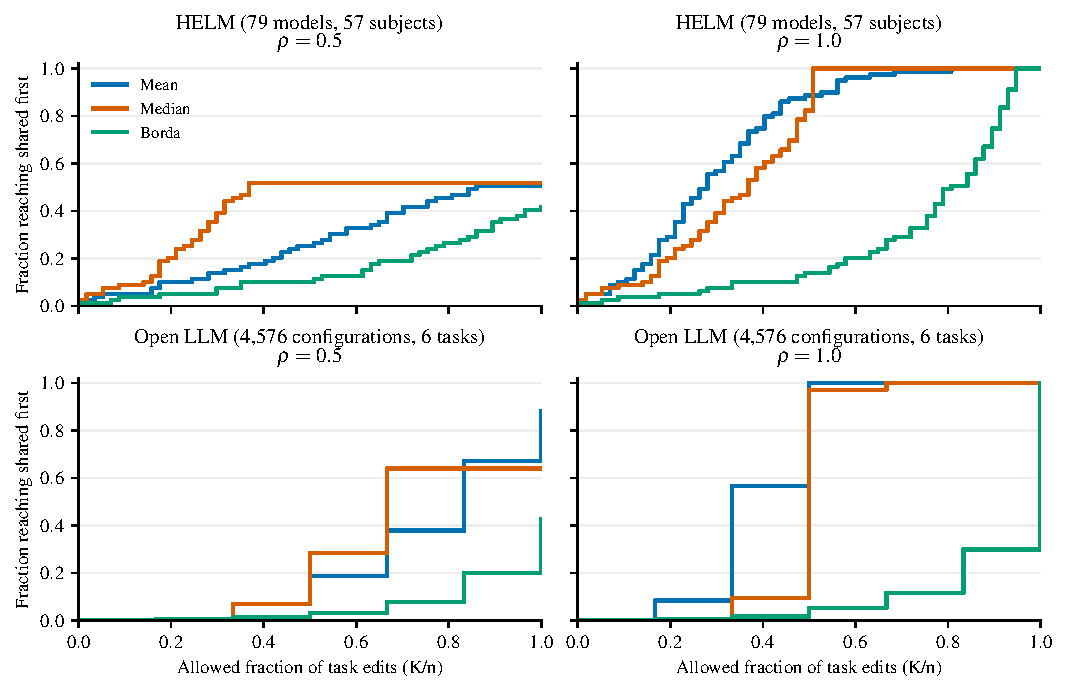
\includegraphics[width=\textwidth]{artifacts/figures/feasibility/plot.pdf}
\caption{All-target shared-first success versus edited-task budget. Infeasible targets remain in the denominator. Thus each curve distinguishes support efficiency from the maximum attainable fraction. A perfect-score ceiling is a structural stress test, not a demonstrated training capability.}
\label{fig:success}
\end{figure*}
At full headroom every target can win under every shared-first rule, as required by setting all target coordinates to 1. Nevertheless, their costs differ: median task counts are 16, 21, and 46 for mean, median, and Borda on HELM, and 2, 3, and 6 on Open. These are within-rule medians over all targets, including existing winners. Figure~\ref{fig:success} shows the complete budget curves rather than only those summaries. Borda's ordinal robustness is neither free nor universal: its larger observed task counts coexist with exact synthetic examples where Borda needs fewer edits than a cardinal rule.

\subsection{A Ceiling-Dependent Reversal on Fixed Targets}
\begin{table*}[t]
\caption{Fixed three-rule feasible nonwinner cohorts selected at $\rho=0.5$. Costs are mean optimal task counts, not median statistics. The last column is the paired mean difference $(K_{\rm med}-K_\mu)/n$ and descriptive target-bootstrap interval, with competitors and target IDs held fixed.}
\label{tab:fixed}
\centering\small
\begin{tabular}{llrrr}
\toprule
Panel ($N$) & $\rho$ & $K_{\rm mean}$ & $K_{\rm med}$ & Difference [95\% interval] \\
\midrule
HELM (31) & 0.5 & 24.68 & 11.55 & -0.230 [-0.274, -0.186] \\ 
HELM (31) & 1 & 8.90 & 11.55 & 0.046 [0.033, 0.058] \\ 
Open LLM (1839) & 0.5 & 3.55 & 3.17 & -0.063 [-0.068, -0.059] \\ 
Open LLM (1839) & 1 & 1.81 & 2.76 & 0.159 [0.156, 0.162] \\ 
\bottomrule
\end{tabular}
\end{table*}
Table~\ref{tab:fixed} isolates the effect of ceiling capacity from changes in target membership. Among the same 31 HELM targets, median needs 13.13 fewer edited tasks on average at half headroom, but 2.65 more at full headroom. Among the same 1,839 Open targets, the corresponding differences are $-0.38$ and $+0.95$ tasks. The paired intervals describe the fixed-cohort comparison, not training uncertainty.

The reversal is not solely an average of unrelated target directions: 25 HELM targets and 724 Open targets strictly reverse their individual mean-versus-median support inequalities across these ceilings. Nor is the result created by requiring Borda feasibility. Pairwise mean/median cohorts contain 37 HELM and 2,926 Open nonwinners; their average count differences also change sign, from $-15.03$ to $+3.03$ and from $-0.57$ to $+0.86$, respectively. Saved common-rank strata disclose where feasibility and support differ, without treating rank as an aggregation-independent quality measure.

\begin{figure*}[t]
\centering
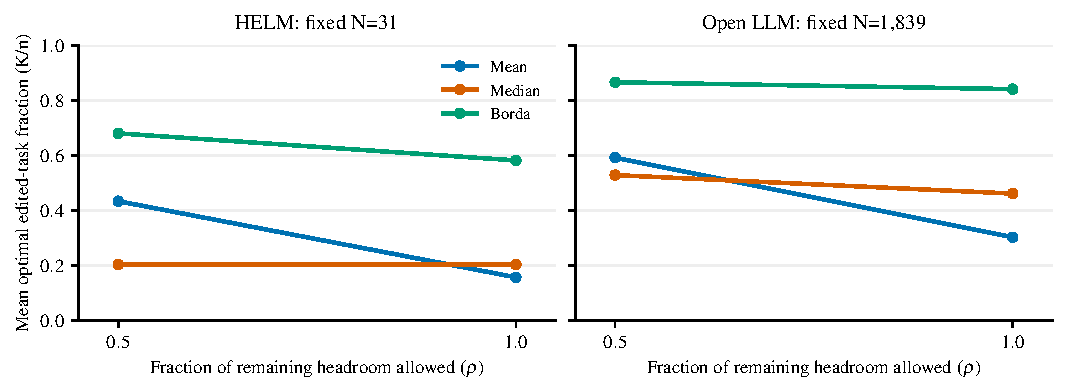
\includegraphics[width=\textwidth]{artifacts/figures/fixed_cohort/plot.pdf}
\caption{Ceiling effects on fixed cohorts from Table~\ref{tab:fixed}. Connecting segments only guide the eye. The HELM median's plateau is predicted by Proposition~\ref{prop:plateau}; increasing capacity reduces mean's required coordinate count. Open's even median can also change its support because the middle pair is coupled.}
\label{fig:fixed}
\end{figure*}
The mechanism is explicit in Figure~\ref{fig:fixed}. On HELM, once a target is median-feasible, its crossing deficit is fixed: extra capacity cannot remove the need for the required number of crossings. Mean can instead concentrate its fixed sum deficit into fewer larger improvements. Open's even median lacks that plateau theorem, yet the fixed-cohort empirical direction still reverses. The theorem explains a sufficient mechanism, not a necessary universal pattern.

\subsection{More Edited Tasks Can Mean Less Score Gain}
For the 77 HELM targets initially nonwinning under both cardinal rules at full headroom, mean's minimum normalized magnitude averages $0.1456$, compared with $0.0344$ for median. All 77 have a smaller median magnitude, and 64 require \emph{more} median task edits while requiring \emph{less} median total score increase. Figure~\ref{fig:magnitude} directly contrasts the two optimizations. The median can pay small local crossing deficits across several subjects, whereas mean must close an aggregate sum deficit. Hence a statement that one rule requires ``more investment'' is incomplete without its cost metric. This comparison uses attained shared-first magnitude optima, not endpoint magnitudes or strict-first infima.

\begin{figure*}[t]
\centering
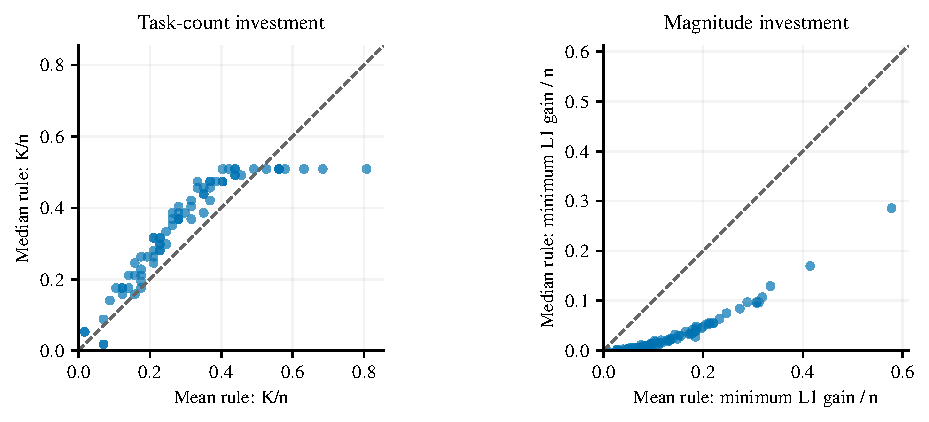
\includegraphics[width=\textwidth]{artifacts/figures/magnitude/plot.pdf}
\caption{Different investment metrics on the same 77 HELM targets, shared first, $\rho=1$. Each point is one target; diagonals mark equality. Left: minimum task-count fractions. Right: independently minimized magnitude, not the amount spent by a ceiling witness. Median costs more tasks for 64 targets but less total gain for every target shown.}
\label{fig:magnitude}
\end{figure*}

\subsection{Sensitivity and Optimization Baselines}
\textbf{Task choice versus optimization.} On feasible half-headroom Borda targets, headroom ordering uses 6.12 excess tasks on average in HELM and 0.32 in Open; random ordering uses 8.19 and 0.49. Thus score headroom alone is not the ordinal investment value. Reachable opponent thresholds and the displaced rivals determine margin gains. The same exact target support is a reference for these heuristics, not evidence of superiority to a training algorithm.

\textbf{Ties and even medians.} Across all three ceilings, unique first changes finite median support in 18 HELM target--ceiling cases and Borda support in three; the Open Borda grid has one feasibility change and four finite support changes. Mean support is unchanged in both snapshots, but this is empirical, not a tie-invariance theorem. On six-task Open, replacing the averaged median with the lower or upper middle statistic changes half-headroom feasibility from 2,927 to 4,163 or 780. The convention is therefore part of the substantive research question.

\textbf{Scales and rosters.} Using official normalized Open scores changes half-headroom feasibility to 4,424 mean, 3,429 median, and 1,969 Borda targets. This changes both the measurement scale and the numerical ceiling intervention, and floor ties can change Borda; it is not a controlled strictly increasing transformation of fixed endpoints. Dropping duplicate score rows leaves cardinal support unchanged on retained targets but changes Borda feasibility in three cases. Availability/unflagged filtering changes Borda feasibility in 45 retained cases, with no cardinal changes. Ordinal analysis depends on the competitor roster even when those competitors' raw scores are not edited. Appendix~\ref{app:sensitivities} gives the consolidated sensitivity table and task-influence caveats.

\section{Discussion and Limitations}
The substantive answer is conditional. With a specified score system, target, ceiling, and winning convention, minimum task count is a well-defined reproducible quantity. Across rules it is not a universal robustness ordering. Our odd-median plateau explains why larger admissible per-task gains can reverse the mean--median comparison even on identical targets. The exact shared-first counterexamples establish non-dominance independently of these particular public tables.

Several limitations constrain interpretation. First, a real update need not stay in an independent upward-only box: task correlations, negative transfer, changing opponents, unknown saturation, and data scarcity are absent. Our computed counterfactuals should not be used to estimate actual development budgets or recommend contamination. Scores are relaxed to a continuum despite finite-test granularity; strict magnitude nonattainment need not survive a discrete score lattice. Second, identical task weights do not imply equal training costs or equal validity, and the six Open coordinates are already task-family summaries, unlike HELM's individual subjects. The numerical fractions $K/n$ are structural comparisons, not evidence that these granularities are interchangeable.

Third, snapshots contain correlated model variants, heterogeneous evaluation protocols, and selection effects. Conditional feasible cohorts are not samples of all models; bootstrap intervals do not fix those issues. We report all-target success curves and roster variants but do not establish causal effects of contamination or uncertainty from test-item resampling. The bounded deletion diagnostic is exploratory and too small to establish task-population generality, including empty feasible cohorts and an explicit parity-preserving HELM deviation.

Fourth, full headroom is an optimistic stress case, and displayed rounding can hide true ties. Numerical tolerance checks validate implementation stability, not unknown score measurement error. No score-rounding perturbation or measurement-noise study was performed. The 57-task solver's matching numerical bounds are not formal optimality certificates. Finally, the independent-source restriction prevents a comprehensive novelty assessment; we disclose that boundary rather than infer what the excluded work might contain.

\section{Conclusion}
Targeted score investment must specify both its admissible gains and its cost. Endpoint reduction turns minimum task count into finite subset selection; minimum magnitude is a separate optimization. On two public score matrices, a fixed-cohort mean--median count comparison reverses when the ceiling changes, and count and magnitude can point in opposite directions. The useful benchmark-design output is therefore a feasibility-aware, convention-specific investment profile, not an unqualified claim that one aggregator prevents strategic improvement. Validating a score-to-training-resource relationship requires a separate intervention study.

\clearpage
\section*{Impact Statement}
This work studies a structural weakness of evaluation summaries using only public aggregate scores. It does not perform model training, supply leaked test data, identify private individuals, or allege misconduct by any model developer. The intended benefit is transparent sensitivity auditing and a clearer distinction between measured performance and general capability. Optimization tools could also help prioritize leaderboard-oriented tuning; their release is limited to counterfactual score analysis and explicitly does not endorse evaluation-set training. Unknown score-data licensing is disclosed, and original sources and retrieval procedures accompany all derived results. This research and its text were produced with AI assistance; the supplied numerical artifacts, tests, source-reading logs, and limitations enable independent checking rather than relying on that assistance as evidence.

\bibliography{paper/references}
\bibliographystyle{paper/template/icml2026}
\clearpage
\appendix
% Input after the references in the ICML 2026 main file.
% Requires only the main file's amsmath, amsthm, booktabs, and hyperref.
% Local theorem environments and labels are independent of the main paper.
% Compiled and audited from the workspace-root paper.tex entrypoint.
\newtheorem{appthm}{Theorem}[section]
\newtheorem{appprop}[appthm]{Proposition}
\newtheorem{applemma}[appthm]{Lemma}

\section{Exact support and magnitude characterizations}
\label{app:theory}\label{app:proofs}

\paragraph{Setting and conventions.}
Let $S\in[0,1]^{m\times n}$, $m\geq2$, $n\geq1$, and fix target $i$, with baseline $x_j=S_{ij}$. Only its row changes, subject to
\begin{equation}
 x_j\leq y_j\leq c_j=x_j+\rho(1-x_j),\qquad 0<\rho\leq1.
 \label{app:box}
\end{equation}
Rival \emph{raw scores} remain fixed. Mean and conventional sample median use equal task weights; for even $n$, the median averages the middle two entries. Borda awards one point per task for beating a rival and half a point for a tie, and sums across tasks. A positive common normalization does not change its winners. Shared first means weakly beating every rival; unique first means strictly beating every rival, with their Borda totals recomputed after edits.

For a fixed rule and winner convention, let $\mathcal W$ be the admissible winning vectors and define
\begin{align}
 K&=\min_{y\in\mathcal W}|\{j:y_j>x_j\}|,\label{app:K}\\
 M&=\inf_{y\in\mathcal W}\frac1n\sum_{j=1}^n(y_j-x_j).
 \label{app:M}
\end{align}
Both values are $+\infty$ when $\mathcal W$ is empty. We explicitly distinguish an attained magnitude minimum from an unattained infimum. $M$ is not defined by imposing support $K$, although the mean and odd-median constructions below also attain or approach it on support-optimal sets. $K$ counts changed coordinates, not money, compute, or an achievable training intervention. The results in this section use exact real inequalities, not numerical tolerances. The clean arguments incorporate the baseline, feasibility, strictness, and counterexample repairs documented in \path{artifacts/theory_audit.md}, Sections 1--5.

\subsection{Endpoint reduction}
\label{app:endpoints}

\begin{applemma}[Endpoint support equivalence]
\label{app:lemma:endpoint}
Put $J=\{j:c_j>x_j\}$ and define $e(A)_j=c_j$ for $j\in A$ and $e(A)_j=x_j$ otherwise. For mean, conventional median, and Borda, under either winner convention,
\begin{equation}
 K=\min\{|A|:A\subseteq J,\ e(A)\in\mathcal W\}.
 \label{app:endpointminimum}
\end{equation}
In particular, a winner using at most $k$ changes exists exactly when a winning endpoint subset of size at most $k$ exists. Any admissible winner exists exactly when the full ceiling vector wins.
\end{applemma}
\begin{proof}
Take a winner $y$ and its actual support $A=\{j:y_j>x_j\}\subseteq J$. Then $e(A)\geq y$ coordinatewise and has exactly support $A$. Mean is coordinatewise nondecreasing. Every order statistic is also nondecreasing: if a coordinatewise increase decreased the $k$th smallest entry from $a$ to $b<a$, the increased vector would have at least $k$ entries at most $b$, whose original entries were also at most $b$, contradicting the original $k$th entry $a$. Thus both middle order statistics, and their average, are nondecreasing. Rival cardinal aggregates are unchanged.

For Borda, use doubled pair points
\[
 p(t,a)=2\mathbf{1}\{t>a\}+\mathbf{1}\{t=a\}.
\]
This is nondecreasing in $t$, and $p(t,a)+p(a,t)=2$. Increasing the target increases its pair points against each rival and decreases that rival's pair points against the target by the same amount; all rival--rival comparisons stay fixed. Consequently every target-minus-rival total margin is nondecreasing, including at ties. Hence $e(A)$ still wins under either convention. Conversely, each endpoint vector is admissible. Raising all coordinates preserves any such victory and proves the final assertion.
\end{proof}
Coordinates outside $J$ cannot be actual edits. Allowing them as binary bookkeeping does not change the minimum, since deleting them leaves the vector unchanged. The lemma does \emph{not} minimize magnitude: a partial edit may win at a smaller $L_1$ cost than its endpoint.

\subsection{Mean: capacity prefixes and magnitude}
\label{app:mean}

\begin{appprop}[Mean characterization]
\label{app:prop:mean}
Let $T=\max_{r\ne i}n^{-1}\sum_jS_{rj}$, $D=nT-\sum_jx_j$, and order the positive capacities $d_j=c_j-x_j$ as $d_{[1]}\geq\cdots\geq d_{[|J|]}$. Put $C_0=0$ and $C_k=\sum_{a=1}^kd_{[a]}$. Then
\begin{align}
 K_{\rm shared}&=\min\{0\leq k\leq|J|:C_k\geq D\},\label{app:meanweak}\\
 K_{\rm unique}&=\min\{0\leq k\leq|J|:C_k>D\}.
 \label{app:meanstrict}
\end{align}
An empty minimum is $+\infty$. For feasible shared victory,
\[
 M_{\rm shared}=\frac{\max(0,D)}n
                 =\max(0,T-\operatorname{mean}(x)),
\]
and this minimum is attained. For unique victory, the complete branches are
\[
 M_{\rm unique}=\begin{cases}
 0,&D<0,\\
 D/n,&D\geq0,\ C_{|J|}>D,\\
 +\infty,&C_{|J|}\leq D.
 \end{cases}
\]
The $D<0$ branch is attained at the baseline; the finite $D\geq0$ branch is never attained.
\end{appprop}
\begin{proof}
Any intervention on at most $k$ coordinates gains at most $C_k$ in the target's task sum; the top-$k$ endpoint subset gains exactly $C_k$. Victory requires total gain at least $D$, or strictly greater than $D$, proving both support formulas, including zero-edit and infeasible cases.

Every shared winner has gain at least $\max(0,D)$. If $D\leq0$, the baseline attains zero. Otherwise take the least $k$ with $C_k\geq D$, fill the first $k-1$ capacities, and give the last coordinate gain $D-C_{k-1}\in(0,d_{[k]}]$. This attains the bound on exactly $K$ coordinates. For unique victory with $D\geq0$, feasibility requires capacity strictly exceeding $D$. Within a support-optimal top-capacity set, distribute total gain $D+\epsilon$ for arbitrarily small positive $\epsilon$. Its normalized cost tends to $D/n$, but every strict winner costs strictly more. If $D<0$, the unchanged row already wins uniquely.
\end{proof}

\subsection{Odd median: crossings, plateau, and all magnitude branches}
\label{app:median}

\begin{appprop}[Odd-median characterization]
\label{app:prop:median}
Let $n=2h-1$ and $T=\max_{r\ne i}\operatorname{median}(S_r)$. For shared first define
\begin{align*}
 q_{\geq}&=|\{j:x_j\geq T\}|,&
 R_{\geq}&=\{j:x_j<T\leq c_j\},\\
 r_{\geq}&=\max(0,h-q_{\geq}).
\end{align*}
For unique first, recompute instead
\begin{align*}
 q_{>}&=|\{j:x_j>T\}|,&
 R_{>}&=\{j:x_j\leq T<c_j\},\\
 r_{>}&=\max(0,h-q_{>}).
\end{align*}
For either convention $\diamond\in\{\geq,>\}$,
\[
 K_\diamond=\begin{cases}
 r_\diamond,&|R_\diamond|\geq r_\diamond,\\
 +\infty,&|R_\diamond|<r_\diamond.
 \end{cases}
\]
In the feasible case, sort the boundary costs $T-x_j$ over $R_\diamond$ increasingly as $a^\diamond_{[1]},\ldots$. Then
\begin{equation}
 M_\diamond=\frac1n\sum_{a=1}^{r_\diamond}a^\diamond_{[a]}.
 \label{app:mediancost}
\end{equation}
The empty sum is zero. Shared magnitude is attained; unique magnitude is attained exactly when $r_{>}=0$, i.e., the baseline is already a unique winner. If infeasible, $M_\diamond=+\infty$, not the finite expression in \eqref{app:mediancost}.
\end{appprop}
\begin{proof}
An odd median is at least $T$ exactly when at least $h$ entries are at least $T$. Initially $q_{\geq}$ qualify. Each new qualifying entry requires one edit from $R_{\geq}$; an upward edit cannot remove an existing qualifying entry. Thus at least $r_{\geq}$ crossings are necessary, and making any $r_{\geq}$ eligible entries equal to $T$ suffices. This proves support and feasibility, including baseline winners. Every shared winner must pay the deficits of at least $r_{\geq}$ eligible entries, whose sum is bounded below by the cheapest such deficits. Editing those cheapest entries exactly to $T$ attains \eqref{app:mediancost} on support $K$.

For strict victory, a median exceeds $T$ exactly when at least $h$ entries exceed it. Entries equal to $T$ do not initially qualify, and a ceiling equal to $T$ cannot qualify. Applying the same count with $q_>$ and $R_>$ proves the strict support formula. If $r_{>}=0$, no edit is needed. Otherwise every winner must newly qualify at least $r_>$ entries, paying strictly more than the sum of their boundary deficits and hence strictly more than \eqref{app:mediancost}. Conversely, for the cheapest $r_>$ strict candidates, set $y_j=T+\epsilon_j$ with $0<\epsilon_j<c_j-T$. Sending these positive increments to zero approaches the bound on exactly support $K$; no winner attains it.
\end{proof}

\paragraph{Precise plateau statement.}
Holding $S$, target, and winner convention fixed, $q_\diamond$ and $r_\diamond$ do not depend on $\rho$. Eligibility, and hence feasibility, can change. Therefore $K$ is constant \emph{on the feasible $\rho$ domain}, not necessarily finite for every cap. A shared crossing with $x_j<T$ requires
\[
 \rho\geq\frac{T-x_j}{1-x_j};
\]
a strict crossing with $x_j\leq T<1$ requires strict inequality. Unique victory at $T=1$ is impossible. Changing the task cohort, rivals, or median convention does not fall under this plateau claim.

\paragraph{Boundary checks and even medians.}
For $x=(1,1,1)$ against $(0,0,0)$, $h-q_{\geq}=-1$, but the correct cost and support are zero: the nonnegative deficit is essential. For $x=(1/2,1/2,0)$ against $(1/2,1/2,1/2)$ at $\rho=1$, shared $K=0$ whereas unique $K=2$, with unattained magnitude infimum zero. These are the audit's baseline and strict-count witnesses. The crossing formula is not valid for the average-middle-pair median at even $n$. Lemma~\ref{app:lemma:endpoint} still applies, so endpoint enumeration is exact; six tasks require only $2^6=64$ subsets.

\begin{applemma}[Continuous-cardinal strict nonattainment]
\label{app:lemma:nonattainment}
For mean or conventional median, including even $n$, if the baseline is not a unique winner but unique victory is feasible, the magnitude infimum is not attained, even on any fixed winning nonempty actual support.
\end{applemma}
\begin{proof}
Both aggregates are continuous. For a strict winner $y$, the path $x+t(y-x)$ remains admissible. For some $t<1$ sufficiently close to one its aggregate still exceeds the fixed rival threshold, while its positive magnitude is multiplied by $t$. Positive $t$ preserves actual support. Thus every strict winner can be made strictly cheaper.
\end{proof}

\subsection{Borda: changing rivals, integer covering, and safe pruning}
\label{app:borda}

\begin{appprop}[Exact Borda support program]
\label{app:prop:borda}
Let $B_r$ denote each row's baseline doubled Borda total. On task $j$, define the target endpoint gain $g_j$ and rival $r$'s endpoint loss $\ell_{rj}$. Then $\ell_{rj}\in\{0,1,2\}$, $g_j=\sum_{r\ne i}\ell_{rj}$, and the exact support problem is
\begin{equation}
 \begin{aligned}
 \min_{z}\quad &\sum_{j\in J}z_j\\
 \text{subject to}\quad
 &\sum_{j\in J}(g_j+\ell_{rj})z_j
       \geq B_r-B_i+\delta,\\
 &z_j\in\{0,1\},
 \end{aligned}
 \label{app:cover}
\end{equation}
with one constraint for each rival $r\ne i$, where $\delta=0$ for shared and $\delta=1$ for unique first. If $B_{\max}=\max_{r\ne i}B_r$, retaining only rivals with $B_r\geq B_{\max}-2n$ preserves this program's feasible subsets and optimum.
\end{appprop}
\begin{proof}
Pairwise complementarity gives
\begin{align*}
 \ell_{rj}&=p(c_j,S_{rj})-p(x_j,S_{rj})\geq0,\\
 g_j&=\sum_{r\ne i}\ell_{rj}.
\end{align*}
Tasks are separable and rival--rival terms never change. Thus an endpoint choice satisfies
\begin{align*}
 B_i(z)&=B_i+\sum_{j\in J}g_jz_j,\\
 B_r(z)&=B_r-\sum_{j\in J}\ell_{rj}z_j.
\end{align*}
Rearranging each winning inequality gives \eqref{app:cover}. All totals are integers, so strict victory is exactly a margin of at least one doubled point. Lemma~\ref{app:lemma:endpoint} transfers the endpoint optimum to all continuous admissible edits. Freezing rival Borda totals would omit $\ell_{rj}$ and solve a different problem.

For pruning, retain an original maximum rival $r_*$ with total $B_{\max}$. Each rival loses at most two doubled points per task, so for every admissible edit
\[
 B_{r_*}(y)\geq B_{\max}-2n.
\]
An omitted rival cannot increase and satisfies
\[
 B_r(y)\leq B_r<B_{\max}-2n\leq B_{r_*}(y).
\]
Beating all retained rivals, weakly or strictly, therefore beats every omitted rival. The converse follows by restriction. Equality at the cutoff is retained; $r_*$ need not remain the leading rival.
\end{proof}

\paragraph{Borda magnitude is a separate problem.}
Continuity-based Lemma~\ref{app:lemma:nonattainment} does not extend to Borda. The audit gives two exact witnesses at $\rho=1$. With target $(0,1)$ and sole rival $(1/2,0)$, the baseline ties, but unique victory has an attained minimum magnitude $1/4$ at $(1/2,1)$. With target $(0,0)$ and rival $(1/2,1)$, shared victory at $(1/2+\epsilon,0)$ approaches infimum $1/4$, but no vector of that magnitude wins: total gain $1/2$ can at best tie the first task while losing the second. Consequently neither endpoint support nor weak winner inequalities imply a Borda magnitude minimum. Endpoint witness costs are not reported as optimized continuous Borda $M$.

\section{Exact synthetic shared-first non-ordering certificates}
\label{app:examples}\label{app:counterexamples}

\begin{appthm}[No universal pairwise shared-first support ordering]
\label{app:thm:nonordering}
For each ordered pair of distinct rules among mean, conventional median, and Borda, an admissible instance has strictly smaller shared-first $K$ for the first rule, with the target initially a nonwinner under every rule.
\end{appthm}

\begin{proof}
The following four matrices, each divided by eight, suffice. Rows are numbered $0,1,2,3$; target row is $0$, tasks are numbered $1,\ldots,5$, and $\rho=1$. Thus every selected target coordinate becomes $8/8$.
\begin{align*}
 8S^A&=\begin{pmatrix}
 7&1&5&4&1\\7&0&8&7&8\\4&1&4&4&1\\8&6&6&5&5
 \end{pmatrix},\\
 8S^B&=\begin{pmatrix}
 4&3&1&5&0\\3&1&3&8&5\\2&0&2&7&6\\7&0&5&6&6
 \end{pmatrix},\\
 8S^C&=\begin{pmatrix}
 1&4&2&1&2\\6&1&8&8&1\\7&7&7&2&6\\8&3&1&8&2
 \end{pmatrix},\\
 8S^D&=\begin{pmatrix}
 6&1&2&5&0\\7&2&8&2&1\\7&7&5&4&5\\8&2&0&0&2
 \end{pmatrix}.
\end{align*}
Table~\ref{app:tab:exactK} states the exact supports; the following lower bounds and witnesses prove all entries without reliance on numerical search.

\begin{table}[t]
\centering
\caption{Exact shared-first supports for four distinct synthetic matrices. These are mathematical examples, not benchmark measurements.}
\label{app:tab:exactK}
\begin{tabular}{lrrr}
\toprule
Matrix & $K_{\rm mean}$ & $K_{\rm median}$ & $K_{\rm Borda}$\\
\midrule
$A$ & 2 & 2 & 3 \\
$B$ & 2 & 3 & 2 \\
$C$ & 3 & 3 & 2 \\
$D$ & 2 & 1 & 2 \\
\bottomrule
\end{tabular}
\end{table}

\emph{Mean certificates.}
In integer eighth-units, target sums are $(18,13,10,14)$ and maximum rival sums $(30,24,29,28)$, giving deficits $(12,11,19,14)$ for $A,B,C,D$. Their descending capacity lists are respectively
\[
 \begin{gathered}
 (7,7,4,3,1),\quad(8,7,5,4,3),\\
 (7,7,6,6,4),\quad(8,7,6,3,2).
 \end{gathered}
\]
The largest insufficient prefixes are $7<12$, $8<11$, $14<19$, and $8<14$; the next prefixes are $14,15,20,15$, which suffice. Endpoint task sets $\{2,5\}$, $\{3,5\}$, $\{1,3,4\}$, and $\{2,5\}$ witness these supports. Proposition~\ref{app:prop:mean} supplies the matching lower bounds for arbitrary edits.

\emph{Median certificates.}
In eighth-units, baseline target medians are $(4,3,2,2)$, rival thresholds are $(7,6,7,5)$, and counts $q_{\geq}$ are $(1,0,0,2)$. Since $h=3$ and every candidate can reach eight, Proposition~\ref{app:prop:median} gives supports $(2,3,3,1)$. Winning endpoint task sets are respectively $\{2,5\}$, $\{1,2,3\}$, $\{1,3,4\}$, and $\{2\}$.

\emph{Borda lower bounds.}
The baseline doubled totals, including every rival, are
\[
 \begin{array}{c|rrrr}
 A&10&21&5&24\\
 B&10&18&12&20\\
 C&9&13&22&16\\
 D&8&16&23&13
 \end{array}.
\]
For baseline leading rivals $r_*=(3,3,2,2)$, the coefficient vectors $g_j+\ell_{r_*j}$ are respectively
\[
 \begin{gathered}
 (3,5,5,7,6),\quad(4,0,8,7,8),\\
 (7,4,5,6,5),\quad(7,8,5,0,8),
 \end{gathered}
\]
and the required margins are $(14,10,13,15)$. For $A$, any two edits gain at most $7+6=13<14$ against this rival. For $B,C,D$, any one edit gains at most $8<10$, $7<13$, and $8<15$, respectively. These necessary constraints and endpoint reduction lower-bound every continuous intervention. The endpoint sets and updated full-rival totals in Table~\ref{app:tab:bordawitness} attain the bounds.

\begin{table}[t]
\centering\small
\caption{Exact Borda upper-bound witnesses from \path{artifacts/theory_audit.md}, Section 5. All totals are doubled points; rival totals are updated. Task indices are one-based.}
\label{app:tab:bordawitness}
\begin{tabular}{lll}
\toprule
Matrix & Endpoint tasks & Updated $(B_0,B_1,B_2,B_3)$\\
\midrule
$A$ & $\{2,4,5\}$ & $(22,18,2,18)$ \\
$B$ & $\{3,5\}$ & $(22,14,8,16)$ \\
$C$ & $\{1,4\}$ & $(18,10,18,14)$ \\
$D$ & $\{2,5\}$ & $(20,12,19,9)$ \\
\bottomrule
\end{tabular}
\end{table}

Every baseline target sum, median, and Borda total is strictly below a rival maximum. Matrix $A$ gives mean $<$ Borda and median $<$ Borda; $B$ gives mean $<$ median and Borda $<$ median; $C$ gives Borda $<$ mean; $D$ gives median $<$ mean. Thus every ordered pair occurs. A single admissible cap $\rho=1$ suffices to refute a universal ordering over instances and caps.
\end{proof}

\paragraph{Provenance and scope.}
The six ordered-pair records in \path{artifacts/counterexamples.json} contain \emph{four}, not six, distinct matrices: $A$ is records 1--2, $B$ records 3--4, $C$ record 5, and $D$ record 6. The exact checker \path{code/counterexamples.py} uses rational arithmetic and shared-first comparisons; its recorded search seed is 916 and candidates examined is 40. Neither search count nor seed supports a probabilistic claim. The displayed matching certificates are the exact witnesses audited in \path{artifacts/theory_audit.md}, Section 5.

These matrices do not establish unique-first non-ordering. Under that convention the audit's support triples become $A=(2,3,3)$, $B=(2,3,2)$, $C=(3,3,3)$, and $D=(2,2,2)$. In particular, $C$'s two largest relevant Borda coefficients sum to 13, whereas uniqueness requires 14; $D$ has only one baseline entry strictly above its median threshold. We claim neither a unique-first non-ordering theorem nor a universal ordering for that convention.

\section{Reproducibility, validation, and sensitivity scope}
\label{app:repro}

\subsection{Pinned inputs, units, and quality control}
\label{app:data}
HELM uses the public MMLU release \texttt{v1.13.0}, with 79 complete valid displayed model configurations and 57 subject exact-match scores. All 79 union rows are retained; no score-row duplicates were found. Run-spec strings and evaluation counts are preserved in \path{artifacts/data_audit.json}. Our equal-subject mean is a constructed ranking, not a reconstruction of an official HELM aggregate.

The Open LLM contents export is pinned to revision
\begin{quote}\small\ttfamily
9c09a7cae43334062a82c\allowbreak{}b164f2ef255013dafa2
\end{quote}
with 4,576 complete valid configurations on IFEval, BBH, MATH Lvl 5, GPQA, MUSR, and MMLU-PRO. Repeated names remain distinct through stable source-row identifiers. There are 54 duplicate-score rows, one flagged row, and 1,683 rows marked unavailable on the hub. These rows remain in the primary analysis; deduplication and available/unflagged filtering are sensitivities, not silent primary exclusions.

\emph{Unit correction to the frozen plan.} The six \texttt{Raw} columns already contain fractions in $[0,1]$ and are \emph{not} divided by 100. Only the official normalized percentage columns are divided by 100. The older wording in \path{todos.md} is superseded by \path{code/prepare.py} and the audit. The mean of those normalized columns reconstructs the exported official average (also divided by 100) with maximum absolute error $1.6653345369377348\times10^{-16}$; this does not equate normalized scores with Raw scores.

Preparation checks unique row identifiers, complete finite scores, and membership in $[0,1]$, without imputation, clipping, or parsing rounded display scores. The recorded exclusion lists are empty for the primary panels and normalized variant. Duplicate and exact-tie diagnostics are retained in \path{artifacts/data_audit.json}; metadata flags are not evidence of misconduct. This score-level QC does not independently verify underlying benchmark examples, model training data, contamination, or the upstream evaluations.

\paragraph{Checksums and access rights.}
\path{data/manifest.json} records source URLs, byte counts, retrieval timestamps, and SHA-256 values for all downloaded data files. For \path{data/raw/contents.parquet}, SHA-256 is
\begin{quote}\small\ttfamily
f13a7061e63133bc8745d89f8c7a56148\allowbreak{}%
584940ede22d3b27e21cad1e078dca5
\end{quote}
For \path{data/raw/helm_summary.json}, it is
\begin{quote}\small\ttfamily
d4eb487e79bcdd7329bdcb10f5116364\allowbreak{}%
c2501842fe5e58da6e0bd717f90ee71e
\end{quote}
The latter is a release-summary checksum, not a checksum of the whole score matrix; individual subject JSON checksums are in the manifest. Data-export licenses are undeclared in the inspected manifests. Public accessibility is not a license grant; redistribution rights must not be inferred from a benchmark paper or a software-release record. No independently verified code-release license is asserted here.

\subsection{Evaluation and numerical validation}
\label{app:validation}
This is a fixed-snapshot analysis, with no new training, inference, fitted hyperparameters, or train/validation/test split. It uses released evaluation scores (HELM run specifications record \texttt{eval\_split=test}); no held-out generalization claim is made. All primary targets and competitors are retained. The main metric is minimum support $K/n$, with infeasibility separate and current shared winners assigned $K=0$. The cap grid is $\rho\in\{0.25,0.5,1\}$, primary $\rho=0.5$; unique first is a separate secondary convention. Comparisons use common feasible nonwinner cohorts, with fixed-cap cohorts and initial-rank strata saved separately. No arbitrary finite penalty substitutes for infeasibility. Borda heuristic baselines use descending headroom and uniform random coordinate orderings with seeds 17, 29, and 43, compared against the support optimum rather than against a trained model.

Mean uses capacity prefixes, odd median uses crossings, and the six-task problems enumerate all 64 endpoint subsets. HELM Borda uses SciPy/HiGHS binary MILP, with a 20-second per-call limit and requested relative gap zero in \path{code/optimize.py}. These are numerical solver settings, not formal certification. The saved validator independently recomputes baseline Borda points, target gains and full-rival losses, admissibility and positive headroom of actual edits, witness costs, all-ceiling infeasibility, cap monotonicity, and shared/unique consistency. Small-instance enumeration tests are in \path{tests/test_optimize.py}.

Cardinal comparisons use tolerance $\tau=10^{-12}$ on aggregate scores: shared victory accepts margin at least $-\tau$ and numerical unique victory requires margin greater than $\tau$. The optimizer's corrected module header, aggregate-level function comparisons, and independent validator use the same convention. Borda uses integer doubled points with exact comparisons of the stored floating-point task scores; this does not recover unknown exact underlying scores.

\path{artifacts/validation_summary.json} reports all 128,915 rows in \path{artifacts/results_*.csv} checked, including 238 nonzero HELM Borda MILP optima with reported gap zero and agreeing numerical lower bounds. Independent witnesses include \emph{all} rivals, not just retained constraints. The validator's full primary cardinal reruns at $\tau=0$ and $10^{-10}$ cover every target, both mean and median, all three caps, and both winner conventions in HELM and Open Raw; none changes $K$ or feasibility. This is not a full tolerance rerun of every sensitivity variant. All recorded checks pass. Neither zero reported MILP gap, numerical bounds, nor floating-point witness validation is a rational-arithmetic optimality certificate. The exact synthetic proofs in Section~\ref{app:examples} are separate evidence.

\paragraph{Uncertainty and multiplicity.}
Paired effect sizes are differences in normalized support on explicitly saved common cohorts. \path{code/summarize.py} produces descriptive 95\% target-bootstrap percentile intervals, using 2,000 resamples for each seed 17, 29, and 43. Reported pooled intervals use the combined bootstrap means; per-seed intervals are also saved. Competitor matrices remain fixed. These intervals do not quantify uncertainty over future models, tasks, training runs, or score measurement. There are no significance tests or multiple-testing-adjusted claims; the intervals are marginal descriptive summaries, not simultaneous confidence guarantees.

\subsection{Sensitivity and task-influence limitations}
\label{app:sensitivity}\label{app:sensitivities}
\begin{table*}[t]
\caption{Open LLM sensitivity at half headroom, shared first. $N$ is the retained identical-target cohort. Changed $K$ counts finite--finite changes only; feasibility changes are reported separately in the CSV.}
\label{app:tab:sensitivity}
\centering\small
\begin{tabular}{llrrrr}
\toprule
Variant & Rule & $N$ & Feas. before & Feas. after & Changed $K$\\
\midrule
Normalized & borda & 4576 & 1960 & 1969 & 31 \\ 
Normalized & mean & 4576 & 4030 & 4424 & 574 \\ 
Normalized & median & 4576 & 2927 & 3429 & 680 \\ 
Deduplicated & borda & 4522 & 1936 & 1933 & 3 \\ 
Deduplicated & mean & 4522 & 3990 & 3990 & 0 \\ 
Deduplicated & median & 4522 & 2897 & 2897 & 0 \\ 
Available & borda & 2893 & 1222 & 1263 & 45 \\ 
Available & mean & 2893 & 2536 & 2536 & 0 \\ 
Available & median & 2893 & 1805 & 1805 & 0 \\ 
Median convention & lower median & 4576 & 2927 & 4163 & 403 \\ 
Median convention & upper median & 4576 & 2927 & 780 & 284 \\ 
\bottomrule
\end{tabular}
\end{table*}
Table~\ref{app:tab:sensitivity} and \path{artifacts/sensitivity_summary.csv} compare the official normalized scale, score-row deduplication, available/unflagged competitor roster, and lower/upper even-median conventions at shared first and $\rho=0.5$. Comparisons retain matching target IDs, but roster changes also change Borda competition. The file distinguishes feasibility changes from changed finite support, with mean $K$ differences conditional on both problems being feasible. These interventions are different estimands; the normalized scale and alternative median conventions change both feasibility and support, and therefore do not justify scale- or convention-invariance. The main empirical tables are not repeated here.

The task-influence protocol is saved in \path{artifacts/task_influence_protocol.json}, with target-level results and summary in \path{artifacts/task_influence_results.csv} and \path{artifacts/task_influence_summary.csv}. It selects 12 equally spaced order statistics of the original baseline mean ordering, breaking ties by stable row order, while retaining all competitors. It evaluates all three rules at shared first and $\rho\in\{0.5,1\}$. Rankings, feasibility, and common nonwinner cohorts are recomputed within each deleted-task panel; normalization uses its remaining task count.

For HELM, each panel deletes two subjects, preserving odd parity ($57\to55$). The six preselected alphabetically indexed pairs are abstract algebra/anatomy, college medicine/college physics, high-school biology/chemistry, high-school physics/psychology, logical fallacies/machine learning, and philosophy/prehistory. The planned single-subject deletion was \emph{not} run: its 56-task conventional median is unsupported by the current large-panel analytic route. This is a solver-coverage limitation, not a theorem that even medians are intractable. For Open Raw, all six single-task deletions are evaluated ($6\to5$), changing the median from an average of two middle values to a single middle order statistic. Consequently these two datasets do not share an identical deletion protocol, and Open's result confounds task removal with parity/convention changes.

The summary's \texttt{median\_minus\_mean} is the mean difference in $K/n$ over targets feasible and initially nonwinning under \emph{all three} rules in that panel. At $\rho=0.5$, deleting MATH Lvl 5 or MUSR leaves this Open cohort empty (panels 2 and 4, zero-based); its contrast is undefined, not zero. The GPQA-deletion panel has only one such target. The protocol is a bounded deterministic diagnostic, not random sampling, a comprehensive leave-task-out audit, or uncertainty estimation. No broad robustness-to-task-selection claim follows, even when a sign repeats across panels.

\subsection{Environment and artifact map}
\label{app:files}
\path{artifacts/environment.json} records Python 3.11.15 on Linux x86\_64 with glibc 2.41, NumPy 2.4.6, pandas 3.0.6, SciPy 1.17.1, matplotlib 3.11.2, PyArrow 19.0.1, and pytest 8.3.5. It records 40 visible logical CPUs and one thread used; this is not identification of physical CPU hardware or a runtime claim.

All paths here are relative to \path{/work/}. Raw inputs are under \path{data/raw/}; primary matrices are \path{data/processed/helm.csv} and \path{data/processed/open_raw.csv}, with \path{data/processed/open_norm.csv} and \path{data/processed/open_metadata.csv} supporting sensitivities. The concise script-to-output map is:
\begin{itemize}
 \setlength{\itemsep}{0pt}
 \item \path{code/download.py}: pinned downloads and \path{data/manifest.json}; \path{code/prepare.py}: matrices and \path{artifacts/data_audit.json}.
 \item \path{code/optimize.py} and \path{code/run.py}: \path{artifacts/results_*.csv}, with per-target masks, status, numerical bounds, and endpoint costs.
 \item \path{code/validate.py}: \path{artifacts/validation_summary.json} and \path{artifacts/boundary_cases.csv}; \path{code/counterexamples.py}: \path{artifacts/counterexamples.json}.
 \item \path{code/summarize.py}: \path{artifacts/paired_contrasts.csv}, \path{artifacts/fixed_cohort.csv}, \path{artifacts/cohort_ids.json}, sensitivity summaries, and \path{paper/generated/} tables.
 \item \path{code/task_influence.py}: protocol, results, and summary named above; \path{code/plot.py}: \path{artifacts/figures/}. Run and validation logs remain in \path{artifacts/}.
\end{itemize}
For example, existing local analysis and validation can be regenerated without retrieving literature by the following commands (not executed for this appendix):
\begin{quote}\small
\begin{verbatim}
export OPENBLAS_NUM_THREADS=1
export OMP_NUM_THREADS=1
export MKL_NUM_THREADS=1
python /work/code/prepare.py
python /work/code/run.py
python /work/code/validate.py
python /work/code/summarize.py
python /work/code/task_influence.py
python /work/code/counterexamples.py
python /work/code/plot.py
python -m pytest /work/tests -q
\end{verbatim}
\end{quote}

\section{Restricted literature scope and voluntary checklist}
\label{app:checklist}

\paragraph{Literature policy and incidental exposure.}\label{app:restriction}
The study's literature access was restricted to seven user-allowlisted original works. As documented in \path{sources/access_log.md}, intended reading used original metadata, abstracts, and selected body passages, excluding related-work, reference, and recommendation sections. No topical discovery, citation following, recommendation lookup, or citation-graph search was used. This is a deliberately incomplete literature review: we make no first-of-kind, exhaustive-prior-art, or priority claim.

The log's final scope supersedes its narrower initial retrieval descriptions. It records accidental display of opening introductions on three first PDF pages, four short reference-like heading lines, and approximately 1,000 characters of a software-release change-log preview. Those reference-like lines and the release preview were not expanded, used as evidence, or followed. Cached complete files do not imply complete reading. Because the excluded work was deliberately unspecified, identity-based exclusion cannot be certified; no attempt is made to infer its identity. This appendix uses the supplied local theory and experiment artifacts and adds no web research or new literature claims.

\paragraph{Voluntary reproducibility and ethics checklist.}
The following is a filled study-specific disclosure, not a NeurIPS checklist. The official ICML author instructions require an Impact Statement, included after the main text; they do not provide a separate mandatory PDF paper checklist. This voluntary checklist supplements that requirement.
\begin{itemize}
 \setlength{\itemsep}{1pt}
 \item \textbf{Claims/proofs: Yes, within scope.} Hypotheses, feasibility, zero edits, strict infima, and even-median exclusions are explicit. Exact non-ordering certificates cover shared first only.
 \item \textbf{Data/QC: Yes.} Pins, checksums, units, row identities, exclusions, duplicates, ties, and flag sensitivities are recorded in Section~\ref{app:data} and the manifest/audit.
 \item \textbf{Code: Local artifacts available.} Commands, environment, witnesses, and solver qualifications are provided. Public archival release, a persistent code identifier, and redistribution permissions are not established.
 \item \textbf{Evaluation/baselines: Yes.} Rules, caps, winner conventions, cohorts, infeasibility, and heuristics are disclosed. New training and held-out splits are not applicable.
 \item \textbf{Uncertainty/corrections: Descriptive only.} Bootstrap seeds and procedure are disclosed; no significance, simultaneous coverage, or multiplicity-corrected inference is claimed.
 \item \textbf{Limitations: Yes.} Endpoint costs need not minimize magnitude; strict optima may not exist; rivals' Borda totals change; HELM single-task deletion is unrun and some Open cohorts are empty. Caps need not be realizable training gains.
 \item \textbf{Licenses/privacy: Undeclared / limited scope.} Export licenses are undeclared in inspected manifests. Only public score/configuration metadata are analyzed, not benchmark answers or participant records. No new recruitment or annotation occurs; upstream privacy and institutional-review compliance are not independently audited.
 \item \textbf{Benefits/harms: Qualitatively assessed.} The analysis may improve transparency about leaderboard incentives but may also inform selective benchmark optimization. It provides no operational training attack, evidence of a named model's misconduct, or justification for contaminating evaluations or equating rank with capability.
 \item \textbf{Impact Statement: Main-file requirement.} Authors must retain the required ICML statement in the main source; this voluntary checklist is supplementary, not a substitute.
\end{itemize}

\end{document}
